\chapter{Il Pneumatico}
\label{Pneumatico}
%
\section{Introduzione}
Gli pneumatici sono probabilmente i componenti più complessi di un'auto in quanto combinano decine di componenti che devono essere formati, assemblati e combinati assieme. Il successo del prodotto finale dipende dalla loro capacità di fondere tutti i componenti separati in un prodotto dal materiale coeso che soddisfa le esigenze del conducente \cite{rill}. Gli pneumatici sono caratterizzati da un comportamento altamente non lineare con una dipendenza da diversi fattori costruttivi e ambientali.
%
\section{Geometria dello Pneumatico secondo ETRTO}
Quando si fa riferimento ai dati puramente geometrici, viene utilizzata una forma abbreviata della notazione completa prevista dall'ente di normazione \ac{ETRTO}. Assumendo di avere un pneumatico generico la notazione che identificherà la geometria sarà del tipo $a$/$b$R$c$. Dove:
\begin{itemize}
	\item $a$ rappresenta larghezza nominale del pneumatico nel punto più largo;
	\item $b$ rappresenta percentuale dell'altezza della spalla dello pneumatico in relazione alla larghezza dello stesso;
	\item $c$ rappresenta il diametro dei cerchi ai quali lo pneumatico si adatta.
\end{itemize}
Facendo un esempio, 195/55R16 significherebbe che la larghezza nominale del pneumatico è di circa 195 mm nel punto più largo, l'altezza della spalla dello pneumatico è il 55\% della larghezza, ovvero 107 mm in questo caso, e che il pneumatico si adatta a dei cerchi di 16 pollici di diametro. Con questa notazione è possibile calcolare direttamente il diametro esterno teorico dello pneumatico tramite la seguente:
%
\begin{equation}
\phi_e = \frac{2ab}{25.4}+c \quad \text{[in]} \qquad
\phi_e = 2ab+25.4c \quad \text{[mm]}
\end{equation}
%
\noindent
Riprendendo l'esempio usato sopra, il diametro esterno risulterà dunque 24.44 in o 621 mm.\\
Meno comunemente usato negli Stati Uniti e in Europa (ma spesso in Giappone) è una notazione che indica l'intero diametro del pneumatico invece delle proporzioni dell'altezza della parete laterale, quindi non secondo \ac{ETRTO}. Per fare lo stesso esempio, una ruota da 16 pollici avrebbe un diametro di 406 mm. L'aggiunta del doppio dell'altezza del pneumatico (2$\times$107 mm) produce un diametro totale di 620 mm. Quindi, un pneumatico 195/55R16 potrebbe in alternativa essere etichettato 195/620R16.\\
Anche se questo è teoricamente ambiguo, in pratica queste due notazioni possono essere facilmente distinte perché l'altezza della parete laterale di un pneumatico automobilistico è in genere molto inferiore alla larghezza. Quindi, quando l'altezza è espressa come percentuale della larghezza, è quasi sempre inferiore al 100\% (e certamente meno del 200\%). Al contrario, i diametri degli pneumatici del veicolo sono sempre superiori a 200 mm. Pertanto, se il secondo numero è superiore a 200, allora è quasi certo che viene utilizzata la notazione giapponese, se è inferiore a 200 allora viene utilizzata la notazione USA/europea.

\begin{figure}[h]
	\centering
	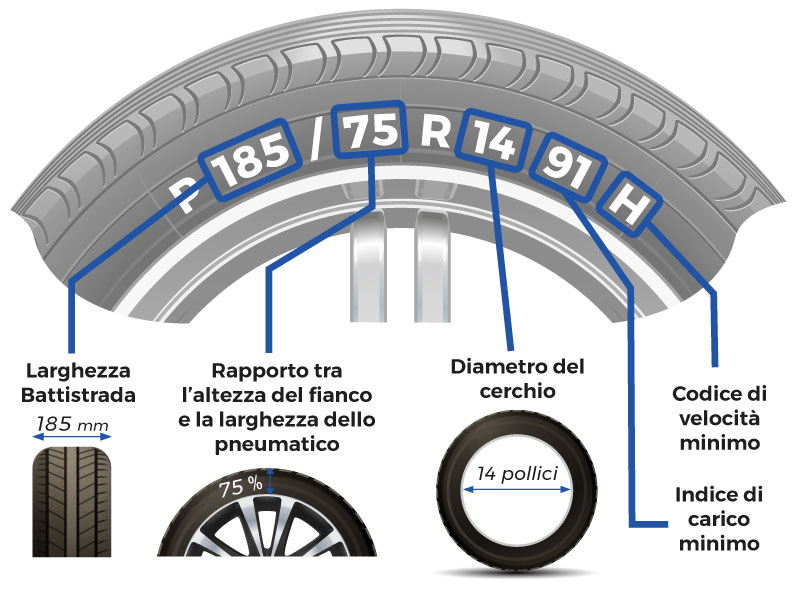
\includegraphics[width=0.7\linewidth]{Figures/tire_measures}
	\caption{Esempio di misure, secondo la notazione ETRTO, riportate sulla spalla dello pneumatico.}
	\label{tiremeasures}
\end{figure}
%
\section{La Modellizzazione dello Pneumatico}
Le forze di contatto tra la superficie stradale e lo pneumatico possono essere descritte completamente da un vettore di forza risultante applicato in un punto specifico dell'impronta di contatto e da una coppia risultante, come illustrato nella \figurename{  \ref{tireforces}}.

\begin{figure}[h!]
	\centering
	\begin{subfigure}{0.4\linewidth}
		$F_x$ \quad forza longitudinale\\
		$F_y$ \quad forza laterale\\
		$F_z$ \quad forza verticale\\
		$T_x$ \quad coppia di sovrasterzo\\
		$T_y$ \quad resistenza al rotolamento\\
		$T_z$ \quad coppia di autoallineamento
	\end{subfigure}
	\begin{subfigure}{0.4\linewidth}
		\centering
		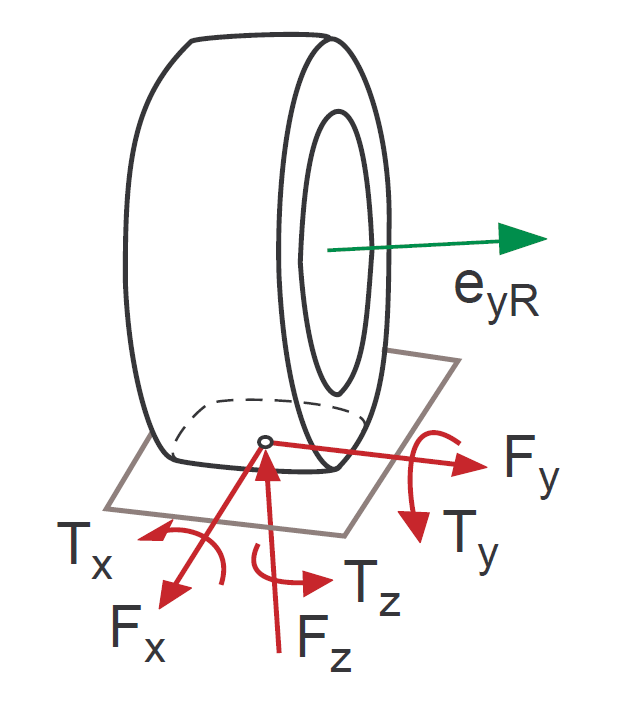
\includegraphics[width=\linewidth]{Figures/tire_forces}
	\end{subfigure}
\caption{Forze e coppie generate dal contatto pneumatico-strada.}
\label{tireforces}
\end{figure}
%
Come componenti cruciali per la movimentazione dei veicoli e il comportamento di guida, le forze degli pneumatici richiedono particolare attenzione soprattutto quando, assieme al comportamento stazionario, anche il comportamento non stazionario dev'essere considerato.

Attualmente, è possibile suddividere i modelli di pneumatico in tre gruppi:
\begin{itemize}
	\item modelli matematici;
	\item modelli fisici;
	\item combinazione dei precedenti.
\end{itemize}

\noindent
La prima tipologia di modello tenta di rappresentare le caratteristiche fisiche del pneumatico attraverso una descrizione puramente matematica. Pertanto questi tipi di modelli partono da un curve caratteristiche ricavate sperimentalmente e cercano di derivare un comportamento approssimativo dall'interpolazione di un grande insieme di dati. Un esempio ben noto di questo approccio è il \textbf{modello di Pacejka} o \textbf{\textit{Magic Formula}} \cite{hans}. Questo tipo di modellazione è adatta per la simulazione di guida dove il comportamento di interesse è per lo più la guidabilità del veicolo e le frequenze di uscita sono ben al di sotto delle frequenze di risonanza della cintura dello pneumatico. I modelli fisici o i modelli ad alta frequenza, come i modelli agli elementi finiti, sono in grado di rilevare fenomeni di risonanza a frequenza più elevata. Ciò permette di valutare la confortevolezza di guida di un veicolo. Dal punto di vista del calcolo, i modelli fisici complessi richiedono molto tempo al calcolatore per essere risolti, nonché di molti dati. Al contrario dei più veloci modelli matematici, che però richiedono un'accurata pre-elaborazione dei dati sperimentali. La terza tipologia di modelli consiste in un'estensione dei modelli matematici attraverso le leggi fisiche al fine di coprire una gamma di frequenza più ampia.

Il modello di pneumatico sviluppato nel modello di veicolo e il tipo di interfaccia di pneumatico/strada presentato da \citeauthor{Larcher} in \cite{Larcher} si basa sulla \textit{Magic Formula} 6.2.
%
\section{Il Modello della \textit{Magic Formula}}
%
\subsection{La \textit{Magic Formula}}
Uno dei modelli di pneumatici più utilizzati è il cosiddetto modello \textit{Magic Formula} sviluppato da \citeauthor{bakker} in \cite{bakker}. Questo modello è stato poi rivisto e l'ultima versione è riportata in \cite{hans}. Il modello \textit{Magic Formula} consiste in una pura descrizione matematica del rapporto input-output del contatto pneumatico-strada. Questa formulazione collega le variabili di forza con lo slip rigido del corpo che vengono trattati nelle sezioni successive. La forma generale della funzione di descrizione può essere scritta come:
%
\begin{equation}
y(x) = D\sin\{C\arctan[B(x + S_h ) - E(B(x + S_h ) - \arctan(B(x + S_h )))]\} + S_v
\end{equation}
%
dove:
\begin{itemize}
	\item $B$ rappresenta il fattore di rigidezza;
	\item $C$ rappresenta il fattore di forma;
	\item $D$ rappresenta il falore massimo della forza o coppia;
	\item $E$ rappresenta il fattore di curvatura;
	\item $S_v$ rappresenta lo spostamento in verticale della curva caratteristica;
	\item $S_h$ rappresenta lo spostamento in orizzontale della curva caratteristica.
\end{itemize}
e dove $y(x)$ può essere la forza longitudinale $F_x$ , la forza laterale $F_y$ o la coppia di autoallineamento $M_z$, mentre $x$ è la componente di slip corrispondente. In \figurename{ \ref{pacejka}} sono illustrate le curve caratteristiche generiche degli pneumatici derivate con il metodo della \textit{Magic Formula}.
%
\begin{figure}[h]
	\centering
	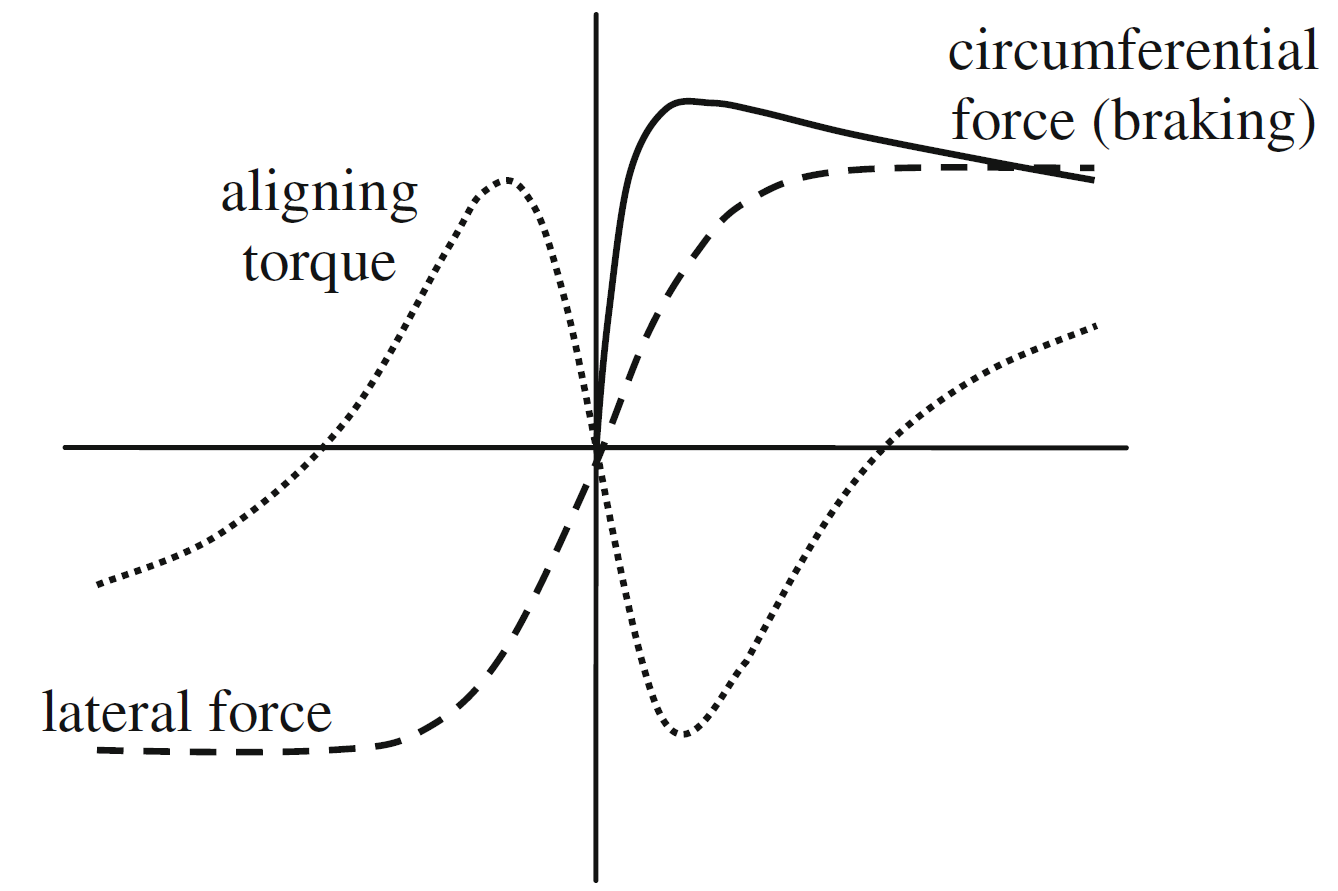
\includegraphics[width=0.58\linewidth]{Figures/pacejka}
	\caption{Curve caratteristiche generiche degli pneumatici derivate con il metodo della \textit{Magic Formula}}
	\label{pacejka}
\end{figure}

\subsection{Contatto con la Superficie Stradale}
La posizione e l'orientamento della ruota in relazione al sistema fissato a terra sono dati dalla terna di riferimento del vettore ruota $RF_{wh_{i}}$, che viene calcolata istante per istante risolvendo le equazioni dinamiche del sistema ottenuto nel Capitolo 2 in \cite{Larcher}. Supponendo che il profilo stradale sia rappresentato da una funzione arbitraria a due coordinate spaziali del tipo: 
%
\begin{equation}
z=z(x,y)
\end{equation}
%
su una superficie irregolare, il punto di contatto $P$ non può essere calcolato direttamente. Così, come prima approssimazione siamo in grado di identificare un punto $P^\star$, che è definito come una semplice traslazione del centro ruota $M$:
%
\begin{equation}
P^\star = M-R_0\textbf{\textit{e}}_{zC}
\begin{bmatrix}
x^\star\\
y^\star\\
z^\star
\end{bmatrix}
\end{equation}
%
dove $R_0$ è il raggio dello pneumatico indeformato e $\textbf{\textit{e}}_{zC}$ è il vettore unitario che definisce l'asse $z_c$ del sistema di riferimento del vettore ruota.

\begin{figure}[h]
	\centering
	\begin{subfigure}{0.45\linewidth}
		\centering
		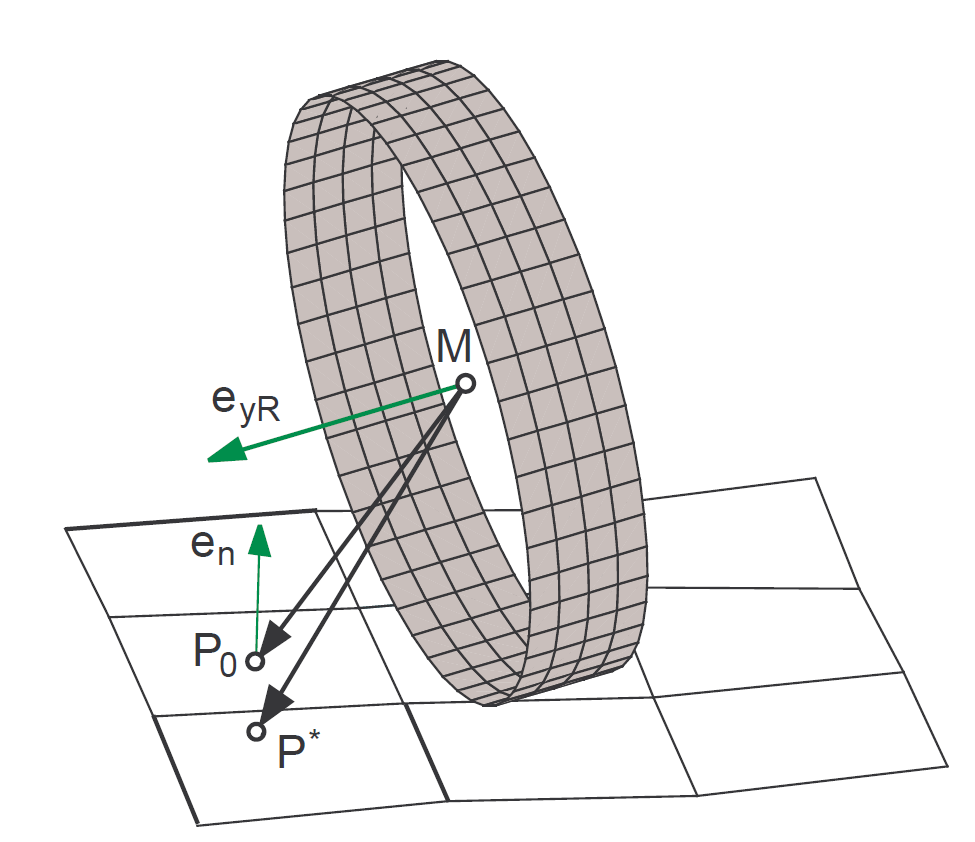
\includegraphics[width=\linewidth]{Figures/contact_geometry_1}
	\end{subfigure}
	\begin{subfigure}{0.35\linewidth}
		\centering
		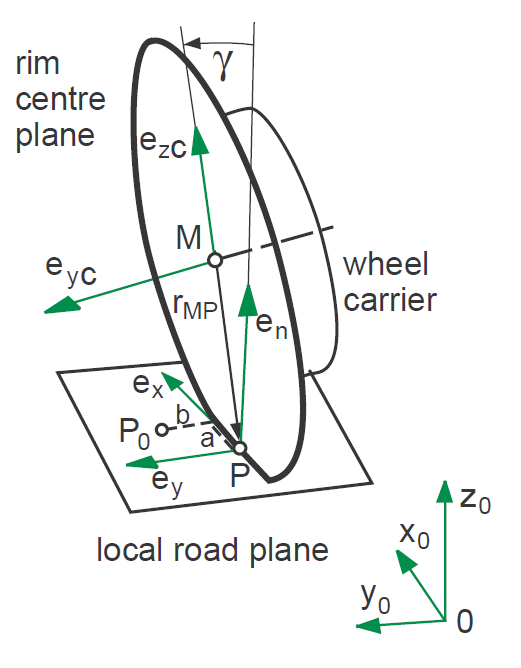
\includegraphics[width=\linewidth]{Figures/contact_geometry_2}
	\end{subfigure}
	\caption{Geometria del contatto pneumatico-strada.}
	\label{contactgeometry}
\end{figure}
%
\noindent
La prima stima del sistema di riferimento del punto di contatto $RF_{PC^\star}$ è una terna con origine in $P^\star$ e orientazione degli assi definiti dall'orientazione del sistema di riferimento della ruota.
%
\begin{equation}
RF_{PC^\star} = \left[
\begin{array}{ccc|c}
& & & x^\star\\
\multicolumn{3}{c|}{\multirow{3}{*}{\raisebox{20mm}{\scalebox{1.5}{$[R_{RF_{wh}}]$}}}} & y^\star\\
& & & z^\star\\ \hline
0 & ~~0 & 0 & 1
\end{array}\right]
\end{equation}\\
%
Ora, i vettori di unità $\textbf{\textit{e}}_x$ ed $\textbf{\textit{e}}_y$, che descrivono il piano locale nel punto $P$, possono essere ottenuti dalle seguenti equazioni:
%
\begin{equation}
\textbf{\textit{e}}_x = \frac{\textbf{\textit{e}}_{yC}\times\textbf{\textit{e}}_{n}}{|\textbf{\textit{e}}_{yC}\times\textbf{\textit{e}}_{n}|}
\qquad
\textbf{\textit{e}}_{y} = \textbf{\textit{e}}_{n}\times\textbf{\textit{e}}_{x}
\label{terna}
\end{equation}
%
Al fine di ottenere una buona approssimazione del piano strada locale in termini di inclinazione longitudinale e laterale, sono stati utilizzati i quattro punti di campionamento $(Q^\star_1, Q^\star_2, Q^\star_3, Q^\star_4)$ che sono rappresentati graficamente in \figurename{ \ref{localtrack}}. I punti di campionamento sono definiti sul sistema di riferimento temporaneo del punto di contatto $RF_{PC^\star}$ e lo spostamento longitudinale e laterale sono definiti dall'origine, ovvero lo stesso $P^\star$. I vettori di spostamento sono definiti come:
%
\begin{equation}
\begin{split}
_{PC^\star}\textbf{\textit{r}}_{Q^\star_{1,2}} = \pm \Delta x \\
_{PC^\star}\textbf{\textit{r}}_{Q^\star_{3,4}} = \pm \Delta y
\end{split}
\end{equation}
%
e quindi, i quattro punti di campionamento sono:
%
\begin{equation}
\begin{split}
_{P^\star}\textbf{\textit{r}}_{Q^\star_{1,2}} = P^\star \pm \Delta x \textbf{\textit{e}}_{xPC^\star} \\
_{P^\star}\textbf{\textit{r}}_{Q^\star_{3,4}} = P^\star \pm \Delta y \textbf{\textit{e}}_{yPC^\star}
\end{split}
\end{equation}
%
Al fine di campionare l'impronta di contatto nel modo più efficiente possibile, le distanze di $\Delta x$ e $\Delta y$, dell'equazione precedente, vengono regolate in base al raggio del pneumatico indeformato $R_0$ e alla larghezza del pneumatico $B$. I valori di queste due quantità possono essere trovate in letteratura e sono $\Delta x = 0.1 R_0$ e $\Delta x = 0.3 B$. Attraverso questa definizione, si può ottenere un comportamento realistico durante la simulazione.

\begin{figure}[h]
	\centering
	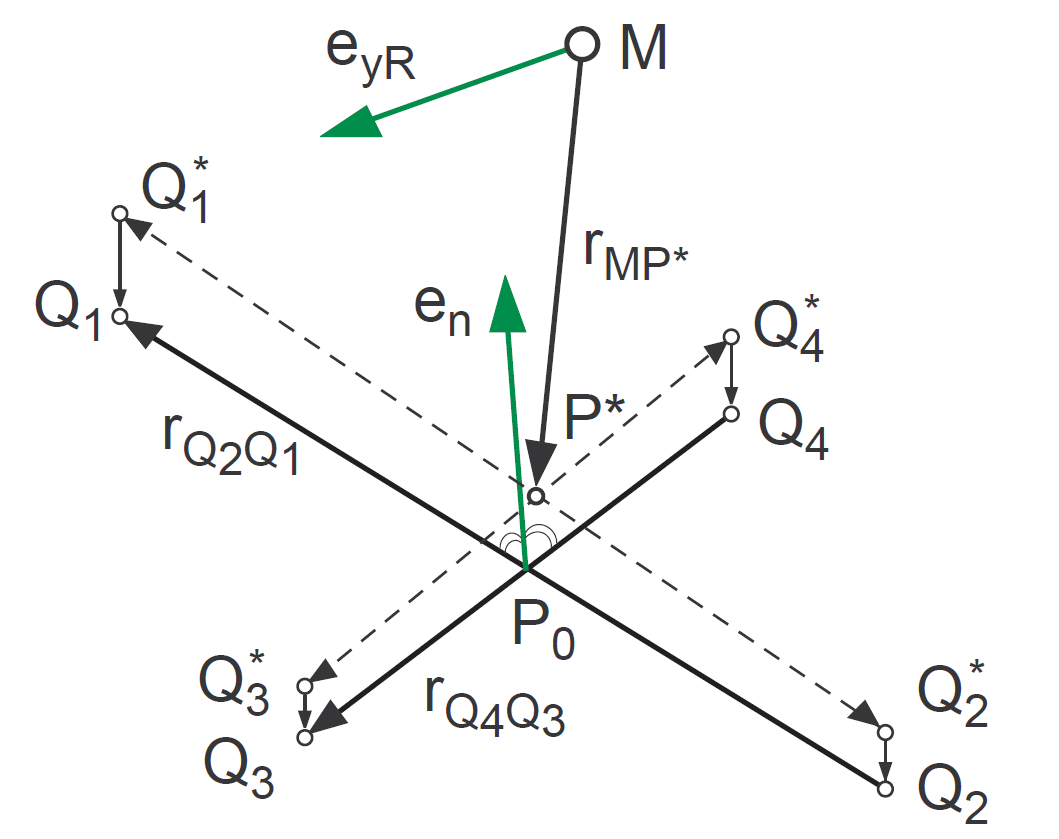
\includegraphics[width=0.5\linewidth]{Figures/local_track}
	\caption{Punti campionati nel piano locale della superficie stradale.}
	\label{localtrack}
\end{figure}
%
\noindent
Ora la componente $z$ in corrispondenza dei quattro punti campione viene valutata attraverso la funzione $z(x,y)$ precedentemente definita. Quindi, aggiornando la terza coordinata dei punti di campionamento $Q^\star_i$, otteniamo i corrispondenti punti campione $Q_i$ sulla superficie della pista locale. La linea fissata dai punti $Q_1$, $Q_2$ e rispettivamente $Q_3$, $Q_4$, può ora essere utilizzata per definire la normale al piano strada locale (\figurename \ref{localplane}). Pertanto, il vettore normale è definito come:
%
\begin{equation}
\textbf{\textit{e}}_n = \frac{\textbf{\textit{r}}_{Q_1 Q_2} \times \textbf{\textit{r}}_{Q_4 Q_3}}{|\textbf{\textit{r}}_{Q_1 Q_2} \times \textbf{\textit{r}}_{Q_4 Q_3}|}
\end{equation}

%
dove sono $\textbf{\textit{r}}_{Q_2 Q_1}$ e $\textbf{\textit{r}}_{Q_4 Q_3}$ sono i vettori che puntano rispettivamente da $Q_1$ a $Q_2$ e da $Q_3$ a $Q_4$. Applicando l'equazione \ref{terna} è ora possibile calcolare i vettori unitari $\textbf{\textit{e}}_{x}$ e $\textbf{\textit{e}}_{y}$ del piano di locale del punto di contatto. Il punto di contatto $P$ si ottiene aggiornando le coordinate del primo punto di prova $P^\star$, con il valore medio delle tre coordinate spaziali dei quattro punti campione.
%
\begin{equation}
P = \frac{1}{4}\begin{bmatrix}
\sum_{i=1}^{4} x_i \\
\sum_{i=1}^{4} y_i \\
\sum_{i=1}^{4} z_i
\end{bmatrix}
\end{equation}
%
Infine possiamo mettere assieme tutte le componenti del piano di riferimento del punto di contatto finale ottenendo:
%
\begin{equation}
RF_{PC} = \left[
\begin{array}{ccc|c}
& & & x_P\\
\multirow{3}{*}{\raisebox{20mm}{\scalebox{1.5}{$\left[\textbf{\textit{e}}_x\right]$}}} & \multirow{3}{*}{\raisebox{20mm}{\scalebox{1.5}{$\left[\textbf{\textit{e}}_y\right]$}}} & \multirow{3}{*}{\raisebox{20mm}{\scalebox{1.5}{$\left[\textbf{\textit{e}}_z\right]$}}} & y_P\\
& & & z_P\\ \hline
0 & 0 & 0 & 1
\end{array}\right]
\end{equation}\\
Attraverso questo approccio, la normale del piano strada locale $\textbf{\textit{e}}_{n}$ insieme al punto di contatto locale $P$, sono in grado di rappresentare l'irregolarità della strada in modo soddisfacente. Come accade in realtà, bordi taglienti o discontinuità del manto stradale saranno smussate da questo approccio. Alcuni casi dimostrativi sono illustrati nella \figurename{  \ref{localplane}}.

\begin{figure}[h]
	\centering
	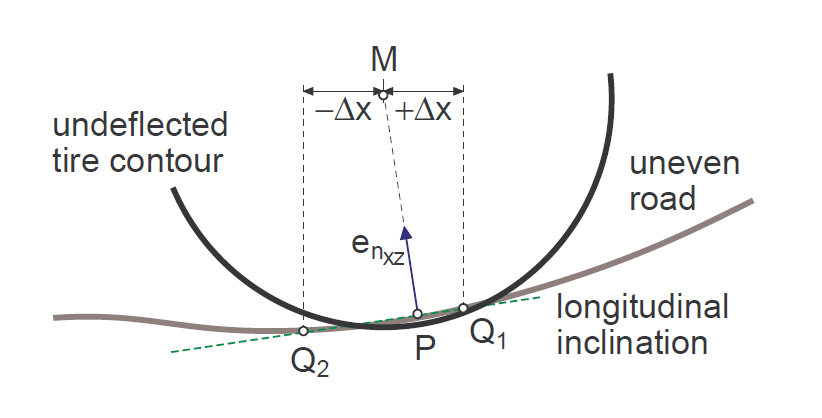
\includegraphics[width=\linewidth]{Figures/local_plane}
	\caption{Inclinazione longitudinale e laterale del piano strada locale.}
	\label{localplane}
\end{figure}